\documentclass[12pt,a4paper]{article}% 

\usepackage{blindtext}
\usepackage{graphicx}
\usepackage{enumitem}
\usepackage{xcolor}
\usepackage{tikz}
\usepackage{algorithm}
\usepackage{textcomp}
\usepackage[noend]{algorithmic}
\usepackage{listings}
	\lstset{
		frame=tb, % draw a frame at the top and bottom of the code block
		tabsize=4, % tab space width
		showstringspaces=false, % don't mark spaces in strings
		numbers=left, % display line numbers on the left
		commentstyle=\color{green}, % comment color
		keywordstyle=\color{blue}, % keyword color
		stringstyle=\color{red} % string color
	}

\usepackage [english]{babel}
\usepackage [autostyle, english = american]{csquotes}
\MakeOuterQuote{"}



\newcommand{\TITLE}[1]{\item[#1]}
\renewcommand{\algorithmiccomment}[1]{$/\!/$ \parbox[t]{4.5cm}{\raggedright #1}}
\newbox\fixbox
\renewcommand{\algorithmicdo}{\setbox\fixbox\hbox{\ {} }\hskip-\wd\fixbox}
\newcommand{\algcost}[2]{\strut\hfill\makebox[1.5cm][l]{#1}\makebox[4cm][l]{#2}}
\usetikzlibrary{arrows,automata,positioning}

\begin{document}
	
	
	\begin{titlepage}
	\title{
\includegraphics[width=0.38 \textwidth]{./NIT_Silchar_logo.png}\\\textbf{\large NATIONAL INSTITUTE OF TECHNOLOGY, SILCHAR}\\\textbf{{\large Department of Computer Science and Engineering}}\\\bigskip {\large Project Report on,}\\\bigskip\textbf{{\normalsize "APPLICATION OF DETERMINISTIC FINITE AUTOMATA IN TEXTUAL PATTERN SEARCHING, ITS PROPERTIES AND EQUIVALENCE WITH NON-DETERMINISTIC FINITE AUTOMATA" }}}
	\author{Subject : Theory of Computation (CS-$204$)\\\\ Under the Supervision of\\\textbf{Dr. Shyamapada Mukherjee} \\\\ Submitted by,\\Name : Arvinder Singh\\Scholar ID : 18-1-5-126}
	\date{\today}
	\clearpage\maketitle
	\thispagestyle{empty}
	\end{titlepage}
	
	\begin{center}
		\textbf{\large ABSTRACT}
	\end{center}
    \begin{flushleft}  \fontsize{12pt}{18pt}\selectfont
		"In this report, I have tried to give a concise overview on one of the applications of finite automata in the realm of textual pattern searching.\\\bigskip Pattern searching is an important problem in computer science. When we search for a word or formally string in notepad, browser, database or in any word processor; pattern searching algorithms are used to show the search results. I have done some in depth mathematical analysis related to time complexity of the same. Also, a C++ program demonstration of  how we can build the finite automata for real life application. \\\bigskip I have also described some properties of DFA in sufficient detail.\\\bigskip Later in the project I have shown equivalence of the DFA we made with another NFA.\\\bigskip This project is developed using one of the open source software \LaTeX\\ and programs shown are developed using CodeBlocks IDE and compiled using g++ 17 compiler." 
	\end{flushleft}
	
	\pagebreak
	\tableofcontents
	\cleardoublepage
	\section{Introduction}\label{sec:intro}
	\begin{flushleft}
		\fontsize{12pt}{18pt}\selectfont
		In computer science, string-matching algorithms are an important class of string algorithms that try to find a place where one or several strings (also called patterns) are found within a larger string or text. There are many applications of string matching like in browser, database or searching \textit{text} in word processor. \\\smallskip 
		
		An example of string searching is when the pattern and the searched text are arrays of elements belonging to finite set of alphabet $\Sigma$. $\Sigma$ may belong to human laguage alphabets, for example it may belong to English alphabets \textit{'a'} to \textit{'z'} or binary digits such as $0$ or $1$ represented as $\Sigma = \{0,1\}$.\\\smallskip 
		
		\subsection{Different types of Searching}
		\begin{flushleft} String searching can be of the following types:\\\smallskip
			\begin{itemize}
				\item {Finding one or more occurrences of a single word in a text or string.}
				\item {Searching occurrences of string (set of words) in non contiguous fashion inside another text or string.}
				\item Searching a same word with alternative spellings such as 'color' and 'colour'
			\end{itemize}
		\end{flushleft}
		Here, we use Finite Automata (FA) based algorithm to search for occurrences of a particular string of length $m$ say \textit{'string1'} in another text of length $n$ say \textit{'text1'}. 
		\subsection{Finite state automaton based search}
		\begin{flushleft}
			In a Naïve approach \textit{(discussed in complexity section)} the time complexity may be very inefficient, of the order $\mathcal{O}(m.n)$ which can be drastically improved to $\mathcal{O}(n)$  searching time,  using finite automaton based searching algorithm. This, motivates us to explore this domain.\\\smallskip
			The very nature of the \textit{finite automata}, the transition of its states for every character it encounters makes this algorithm adequate for this application.
		\end{flushleft}
	\end{flushleft}
	\pagebreak
	\section{Background Theory}
	In Theory we would basically discuss, starting from formal mathematical definition of finite automata, idea for the automaton, functioning , construction and finally giving an example to understand the transitions.
		\subsection{Finite automata}
		\begin{flushleft}
			A \textbf{deterministic finite accepter} or \textbf{dfa} say \textit{M} is a $5-tuple$ or quintuple defined by
			\begin{center}
				$M=(Q,\Sigma,\delta,q_0,F)$
			\end{center}
			where,\\\smallskip
			$Q$ is a finite set of \textbf{internal states},\\
			$\Sigma$ is a finite set of symbols called the \textbf{input alphabet},\\
			$\delta : Q \times \Sigma \rightarrow Q$ is a total function called the \textbf{transition function},\\
			$q_0 \in Q$ is the \textbf{initial state},\\
			$F \subseteq Q$ is a set of \textbf{final states}.\\\bigskip
			The transition from one internal state to another are governed by the transition function $\delta$. It can be conveniently expressed as:
			\begin{equation} \label{eq:1}
				\delta(q_i,a)=q_j
			\end{equation}
			The above represents that if the current state was $q_i$, then upon the consumption of an input symbol $a \in \Sigma$, the \textbf{dfa} will go into state $q_j$.\\\bigskip
			Similarly an extended transition function $\delta ^{*} : Q \times \Sigma^{*} \rightarrow Q$ can be introduced which instead of consuming a single symbol or alphabet, consumes an array of symbols called \textit{string}. Here, the change is in the second argument of the \textit{LHS} of eq.$(1)$.\\\bigskip
			Formally, if $\delta(q_i,a)=q_j$ and $\delta(q_j,b)=q_k$, where $a,b \in \Sigma$ then,
			\begin{equation} 
				\delta^{*}(q_i,ab)=q_k
			\end{equation}
			which can be generalized for any arbitrary string \textit{w} as,
			\begin{equation} 
				\delta^{*}(q_i,w)=q_k
			\end{equation}
			Also, the language accepted by a dfa $M=(Q,\Sigma,\delta,q_0,F)$ is the set of all strings on $\Sigma$ accepted by $M$. In formal notation,
			\begin{center}
				$L(M)=\{w \in \Sigma^{*}:\delta^{*}(q_0,w)\in F\}$
			\end{center}
			\pagebreak
		\end{flushleft}
		\subsection{Idea for automaton}
		The basic idea is to build an automaton in which:
		\begin{itemize}
			\item {Each character in the pattern to be matched has a state.}
			\item {Each match sends the automaton into a new state.}
			\item {If all the characters in the pattern has already been matched, the automaton enters the accepting state.}
			\item {Contrary to the above, if the automaton is not in the final state than it will return to a suitable state according to the current state and the input character.\textit{ This returned state reflects the maximum advantage we can take from the previous matching}.}
		\end{itemize}
		\subsection{Working}
		\begin{flushleft}
		In Finite Automata based algorithm, we pre-process the pattern and build a 2-D array that represents a Finite Automata, in terms of implementation. Construction of the finite automata is the main tricky part of this algorithm. Once the finite automata is built, the searching is simple. In search, we simply need to start from the \textit{start} state of the automata and the first character of the \textit{text}. At every step, we consider next character of \textit{text}, look for the next state in the built finite automata and move on to the next state, with respect to the transition function $\delta(q_i,a)=q_j$. If we reach a final state, then the pattern is found in the text and not, otherwise.\\\bigskip
		Given any input string \textit{w}, over the alphabet $\Sigma$, a finite automata,
		\begin{itemize}
			\item{starts reading from \textit{start} state $q_0$, and}
			\item{reads the string \textit{w}, character by character, changing state each character read.}
		\end{itemize}
		When the finite automata is in state $q_i$ and reads character $\sigma \in \Sigma$, it enters state $\delta(q,\sigma)$.\\\bigskip
		The finite automaton
		\begin{itemize}
			\item{\textbf{accepts} the string \textit{w} if it ends up in an accepting state, and}
			\item{\textbf{rejects} \textit{w} if it does not end up in an accepting state.}
		\end{itemize}
		\pagebreak
		\end{flushleft}
		\subsection{Construction}
		\begin{flushleft}
		We construct a finite automata for a pattern $P=p_{1}p_{2}...p_{m}$ in a text $T=t_{1}t_{2}...t_{n}$.
		\begin{itemize}
			\fontsize{12pt}{18pt}\selectfont
			\item{The finite automata will have $m+1$ states, which we number $0,1,...,m$}
			\item{State $q_0$ will be the starting state, and $m$ will be the only accepting state.}
			\item{In general, the finite automata will be in state $k$ if $k$ characters of the pattern have been matched.\\\smallskip 
			In other words, the finite automata is in state $k$ if the $k$ most recently read characters of the \textit{text} match the first $k$ \textit{pattern} characters.}
			\item{If the next \textit{text} character $t_{j+k}$ equals $p_{k+1}$ (\textit{j can be considered as offset}) , we have matched $k+1$ characters, and the finite automata enters state $k+1$.\textit{i.e.,} $\delta(k,p_{k+1})=k+1$.}
			\item{If the next character $t_{j+k}$ differs from $p_{k+1}$, then the finite automata enters a state $0,1,2,...,k$, depending on how many initial characters of the pattern matched text characters ending with $t_{j+k}$.\\\smallskip
			We shift the pattern, right till we obtain a match, or exhaust the pattern.\\\smallskip
			If $\sigma=t_{j+k}\neq p_{k+1}$, then $\delta(k,\sigma)$= largest integer d such that,\\\smallskip \begin{center}
				$t_{j+k-(d-1)} ... t_{j+k-2} t_{j+k-1} t_{j+k} = p_{1} ... p_{d-2} p_{d-1} p_{d}$
			\end{center}
			This makes it appear that $\delta(k,\sigma)$ depends on the subjects as well as the pattern, but recall that to be in state $k$ to begin with we must have a match meaning $t_{j+i}=p_{i+1}$ for $i=0,1,2,...k-1$. }
		
		\end{itemize}
		\pagebreak
		\end{flushleft}
	    \subsection{Finite Automata example}
	    \begin{flushleft}
	    	In this subsection, I have given an example of finite automata construction for recognition of the pattern 'WXAX'.\\\bigskip
	    	Upon following either the transition table or the automata we see that an example string 'WAAX' is rejected, whereas 'WXAX' is accepted.
	    	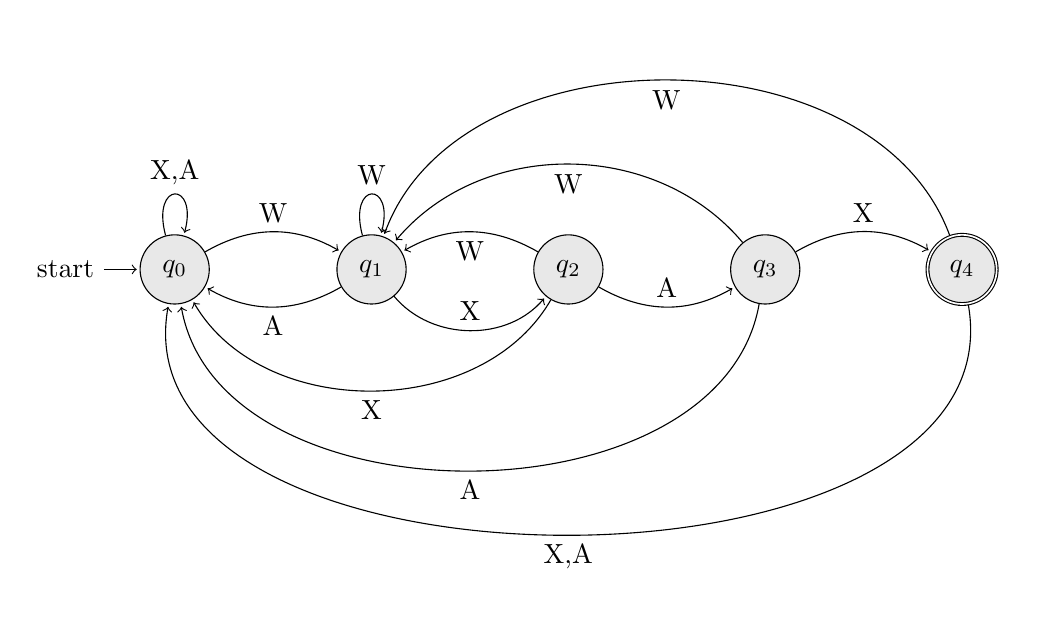
\begin{tikzpicture}[shorten >=1.0pt,node distance=2.5cm,on grid,auto] 
	    	\tikzstyle{every state}=[fill={rgb:black,1;white,10}]
	    	
	    \node[state,initial]   (q_0)                    {$q_0$};
	    \node[state]           (q_1)  [right of=q_0]    {$q_1$};
	    \node[state]           (q_2)  [right of=q_1]    {$q_2$};
	    \node[state]           (q_3)  [right of=q_2]    {$q_3$};
	    \node[state,accepting] (q_4)  [right of=q_3]    {$q_4$};
	    
	    \path[->]
	    (q_0) edge [loop above] node {X,A}  (   )
	    	  edge [bend left]  node {W}    (q_1)
	    (q_1) edge [bend right=50] node {X}    (q_2)
	          edge [loop above] node {W}    (   )
	          edge [bend left]  node {A}    (q_0)
	    (q_2) edge [bend right]  node {W}    (q_1)
	    	  edge [bend left=60]  node {X}    (q_0)
	    	  edge [bend right]  node {A}    (q_3)
	    (q_3) edge [bend right=50]  node {W}    (q_1)
	          edge [bend left]  node {X}    (q_4)
	          edge [bend left=80]  node {A}    (q_0)
	    (q_4) edge [bend right=70]  node {W}    (q_1)
	          edge [bend left=100]  node {X,A}  (q_0);
	    	  
	    	\end{tikzpicture}
	    \\\bigskip
	    \begin{table}[ht]
	    	\centering % used for centering table
	    	\begin{tabular}{c c c c} % centered columns (4 columns)
	    		\hline %inserts double horizontal lines
	    		Present State & W & A & X \\ [0.5ex] % inserts table
	    		%heading
	    		\hline % inserts single horizontal line
	    		$q_0$ & $q_1$ & $q_0$ & $q_0$ \\ % inserting body of the table
	    		$q_1$ & $q_1$ & $q_0$ & $q_2$ \\
	    		$q_2$ & $q_1$ & $q_3$ & $q_0$ \\
	    		$q_3$ & $q_1$ & $q_0$ & $q_4$ \\
	    		$q_4$ & $q_1$ & $q_0$ & $q_0$ \\ [1ex] % [1ex] adds vertical space
	    		\hline %inserts single line
	    	\end{tabular}
    		\caption{Transition Table for finite automata} 
	    \end{table}

    	We can clearly observe from the construction of the above \textit{dfa} that if the length of the string to be recognized is $m$ then, we require a dfa with $m+1$ states in total.\\\smallskip
    	Also, we can observe intuitively the fact that as we move on scanning the text to be scanned for the \textit{string}, for every character we encounter we change the state depending on the transition $\delta$, giving us time complexity of the order $\mathcal{O}(n)$ \textit{(refer to complexity analysis discussed in \textbf{Section} $4$)}.
	    \end{flushleft}
	\pagebreak
	
	
	\section{Algorithm}
	In this section I have given algorithms for answer generation, \textit{i.e.,} generating matches which comprises mainly of the following functions: \textsc{Find-Ans}$(T,P)$, \textsc{Find-Transition-Table}$(P,trans,m)$ and \textsc{Next-State}$(P,m,state,c)$. \bigbreak
	\textbf{Algorithm}
	\begin{itemize}
	\item{\begin{algorithmic}[1]
		\TITLE{\textsc{Find-Ans}$(T,P)$}\COMMENT{$T \rightarrow$ Text, $P \rightarrow$ Pattern }
		\STATE{$m \gets$  $P.\mathit{length}$}
		\STATE{$n \gets$  $T.\mathit{length}$}
		\STATE{initialize  $\mathit{trans}[m+1][|\Sigma|]$}\COMMENT{0 based indexing, quantity inside bracket represents size only}
		\STATE{\textsc{Find-Transition-Table}$(P,trans,m)$}
		\FOR{$i=0$ \TO $n-1$}
		\STATE {$\mathit{state} =\mathit{trans}[state][T(i)] $}
		\IF{$state ==$  $m$}
		\PRINT{("Match found at index = $i-(m-1)$")}
		\ENDIF
		\ENDFOR
	\end{algorithmic}}\bigskip
	\item{\begin{algorithmic}[1]
		\TITLE{\textsc{Find-Transition-Table}$(P,trans,m)$}
		\FOR{$\mathit{state}=0$ \TO $m$}
		\FOR{$\mathit{c}=0$ \TO $|\Sigma|-1$}
		\STATE{ $\mathit{trans}[state][c]$=\textsc{Next-State}$(P,m,state,c)$}
		\ENDFOR
		\ENDFOR
	\end{algorithmic}}\bigskip
	\item{\begin{algorithmic}[1]
		\TITLE{\textsc{Next-State}$(P,m,state,c)$}
		\IF{$state == m$ and $c == P(\mathit{state}) $}
		\RETURN{$\mathit{state}+1$}
		\ENDIF
		\FOR{$\mathit{next=state}$ \TO $1$}
		\IF{$P(\mathit{next}-1)==c $}
		\FOR{$\mathit{i=0}$ \TO $next-2$}
		\IF{$P(\mathit{i})==P(\mathit{state-(next}-1)+1) $}
		\STATE{\textbf{break}}
		\ENDIF
		\ENDFOR
		\IF{$\mathit{i==next-}1$}
		\RETURN{$\mathit{next}$}
		\ENDIF
		\ENDIF
		\ENDFOR
		\RETURN{$0$}
	\end{algorithmic}}
	\end{itemize}
	\begin{flushleft}
		This works absolutely fine while searching for \textit{string} in \textit{text} separated by space.\\ I have also, given a code demonstration in \textbf{Section} $5$ along with the test case demonstrating the same.
	\end{flushleft}
	\pagebreak
	
	
	\section{Complexity Analysis}
	\begin{flushleft}
	Considering the Naïve approach, the time complexity of the algorithm is very poor. Since, this algorithm checks for patterns in the given \textit{text} in iterations. Consider, any general character of the \textit{text} $\sigma$, we start matching \textit{string} from this point, if it succeeds \textit{i.e.,} pattern is found in the \textit{text} then it simply reports it. Otherwise we start checking from the next character in \textit{text}. Thus this gives worst case complexity of $\mathcal{O}(m.n)$ which is indeed poor.\\\bigskip
	On the other hand,the string-matching automaton is very efficient, it examines each character in the text exactly once and reports all the valid shifts of states in \textit{dfa} in $\mathcal{O}(n)$. This implies that search takes $\mathcal{O}(n)$ time since each character is examined once.\\\bigskip
	Observing the algorithms mentioned in the respective algorithm section, we see that the \textsc{Next-State}$(P,m,state,c)$ takes $\mathcal{O}(m^{2})$ to compute next state for a given state and a character say $\sigma$ or say to compute the transition $\delta(q_i,\sigma)$.\\\bigskip
	We compute this,\textit{i.e.,} $\delta(q_i,\sigma)$ for every \textit{state} and character $\sigma$ in the \textsc{Find-Transition-Table}$(P,trans,m)$ function which takes $\mathcal{O}((m+1)|\sigma|)$. However, in total we have,
	\begin{center}
		$\mathcal{O}((m+1)|\sigma|)$.$\mathcal{O}(m^{2})$\\\smallskip
		$=\mathcal{O}(m^{3}|\Sigma|)$
	\end{center}
	Building the transition array\textit{(finite automata)} is a bit expensive as the \textsc{Find-Ans}$(T,P)$ funciton in the algorithm section above takes $\mathcal{O}(m^{3}|\Sigma|)$, where $m$ is the length of the pattern and $|\Sigma|$ is the total possible characters in the \textit{'pattern and the text'}. However, since size $m$ is generally small the overall complexity is not much affected by the cube factor.\\\bigskip
	If we treat number of characters \textit{i.e.,} $|\Sigma|$ as a constant, however it can be as large as $256$(\textit{considering all the ASCII characters}), we have a time complexity of $\mathcal{O}(m^{3})$, which is not bad considering the pattern to be searched to be fairly short(\textit{which is the case in general application}), compared to the actual text to be scanned which is the main concern.\\\bigskip
	So, we can conclude that the overall complexity of the algorithm \textit{i.e.,} construction of finite automata plus searching is $\mathcal{O}(m^{3}+n)$, if $|\Sigma|$ is treated as constant. 
	\end{flushleft}
	\pagebreak
	\section{Code}
	\begin{flushleft}
		Below is a $C++$ code.\\\bigskip
		It consists of all three algorithms exactly as displayed in algorithms section. Further, the code mentioned below is well described with the help of comments.\\\bigskip
	\end{flushleft}
	\begin{lstlisting}[language=C++, caption={C++ code for searching}]
	#include<bits/stdc++.h>
	using namespace std;
	
	int nextState(string pat, int m, int state, int c)
	{
   	  if(state<m && c==pat[state]) return state+1;
 	  for(int nx = state; nx>0; nx--){
	  if(pat[nx-1]==c){
	   int i = 0;
	   for(i=0;i<nx-1;i++)
	    if(pat[i]!=pat[state-(nx-1)+i])
	     break;
	    if(i==nx-1) return nx;
	  }
	 }
	return 0;
	}
	
	void find_trans(string pat, vector<vector<int>> &trans, int m)
	{
	for(int state = 0; state<=m; state++)
	 for(int c = 0; c<256; c++)
	  trans[state][c] = nextState(pat, m, state, c);
	  //comparing all 256 ASCII characters
	  
	}
	
	void find_(string text, string pat)
	{
	int m = pat.length() , n = text.length();
	//Creating a transition table for jumps
	vector<vector<int>> trans(m+1,vector<int> (256));
	//256->represents the no. of characters
	find_trans(pat,trans,m);
	//function call to generate answer for transition table.
	int state = 0;
	//0->represents initial state
	for(int i=0;i<n;i++){
	 state = trans[state][text[i]];
	 //Reading current literal and taking current state
	 if(state = = m) cout<<"Match found at index= "<<i-(m-1)<<endl;
	 }
	}
	//Below is the driver program
	int main()
	{
	string text, pat;
	//Where text,pat-> text and pattern to be scanned for the match
	getline (cin,text);
	getline (cin,pat);
	//User input
	find_(text,pat);
	//function to generate answer as per the algorithm
	}
	\end{lstlisting}
	\begin{flushleft}
	\textsc{Test Cases}\\
    \textbf{Input:}\\\textit{Text}:WXAXAXAXWXAXWXAAXAWXAWXAWXAXAWXWAXWXAXWAX...\\AWXAXWXXWAXXWA\\\textit{Pattern}:WXAX\\
    \textbf{Output:}\\Match found at index= 0\\                                                                                                        
    Match found at index= 8\\                                                                                                       
    Match found at index= 24\\                                                                                                      
    Match found at index= 34\\                                                                                                      
    Match found at index= 42\\\bigskip
    \textbf{Input:}\\\textit{Text}:This is the string to be searched.\\\textit{Pattern}:string\\
    \textbf{Output:}\\Match found at index= 12\\
    
	\end{flushleft}
	\pagebreak
	\section{Equivalence with NFA}
	\begin{flushleft}
		We have seen the deterministic(\textit{dfa}) version of the finite automata, in \textit{dfa} \textit{a unique transition is defined for each state and each input symbol}. Formally, $\delta$ is a total function. This is what makes such automata deterministic. Situations where more than one transition is possible make such automata nondeterministic in nature.\\\bigskip
		However, computers are deterministic in nature and practical realization of \textit{nfa} is impractical. Here, we therefore largely focus on theoretical aspects only. \\\bigskip 
		We will see theoretically how, with \textit{nfa} we would have realized pattern matching \textit{i.e.,} what we just did with \textit{dfa}. Formally,\\\bigskip
		A \textbf{nondeterministic finite accepter} or \textbf{nfa} say \textit{M} is a $5-tuple$ or quintuple defined by
		\begin{center}
			$M=(Q,\Sigma,\delta,q_0,F)$
		\end{center}
		where,\\\smallskip
		$Q$ is a finite set of \textbf{internal states},\\
		$\Sigma$ is a finite set of symbols called the \textbf{input alphabet},\\
		$\delta : Q \times (\Sigma \cup \{\lambda\}) \rightarrow 2^{Q}$ is  the \textbf{transition function},\\
		$q_0 \in Q$ is the \textbf{initial state},\\
		$F \subseteq Q$ is a set of \textbf{final states}.\\\bigskip 
		Here, a transition like the following is also possible,
		\begin{center}
			$\delta(q_i,\sigma)=\{q_u,q_v,...\}, \sigma\in(\Sigma \cup \{\lambda\})$
		\end{center}
		The \textit{dfa} in section $2.5$ can be conveniently expressed with its equivalent \textit{nfa} as follows:\\\bigskip
		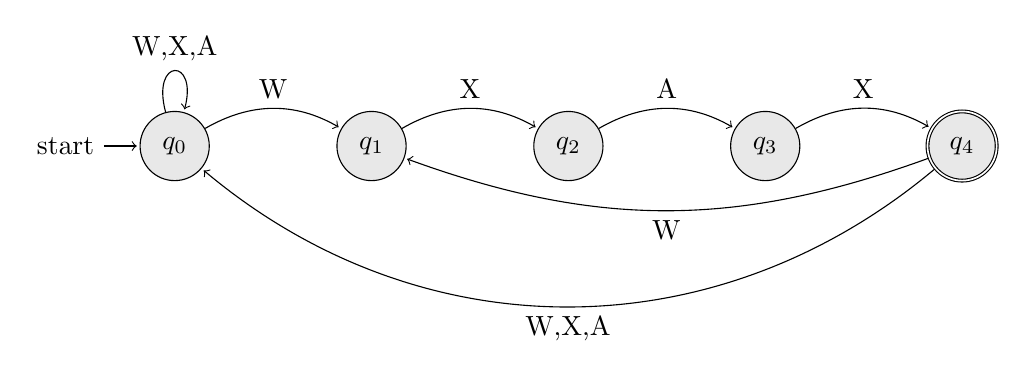
\begin{tikzpicture}[shorten >=1.0pt,node distance=2.5cm,on grid,auto] 
		\tikzstyle{every state}=[fill={rgb:black,1;white,10}]
		
		\node[state,initial]   (q_0)                    {$q_0$};
		\node[state]           (q_1)  [right of=q_0]    {$q_1$};
		\node[state]           (q_2)  [right of=q_1]    {$q_2$};
		\node[state]           (q_3)  [right of=q_2]    {$q_3$};
		\node[state,accepting] (q_4)  [right of=q_3]    {$q_4$};
		
		\path[->]
		(q_0) edge [loop above] node {W,X,A}  (   )
		edge [bend left]  node {W}    (q_1)
		(q_1) edge [bend left] node {X}    (q_2)
		(q_2) edge [bend left]  node {A}    (q_3)
		(q_3) edge [bend left]  node {X}    (q_4)
		(q_4) edge [bend left=20]  node {W}    (q_1)
		edge [bend left=40]  node {W,X,A}  (q_0);
		
		\end{tikzpicture}\\
		\begin{center}
			Tracing the above \textit{nfa} we find that it accepts the string 'WXAX'
		\end{center}
	
    \end{flushleft}
	\pagebreak
	\section{Further Work}
	\begin{flushleft}
		\fontsize{12pt}{20pt}\selectfont
		The string matching algorithm is very efficient and searching only takes $\mathcal{O}(n)$ and construction process of the finite automata takes $\mathcal{O}(m^{3}|\Sigma|)$. We have already discussed this in details in previous sections.\\\bigskip
		The above algorithm is very efficient one but it can be further improved to work in  $\mathcal{O}(m+n)$, this can be done using the idea of longest prefix suffix approach used in \textit{KMP(Knuth–Morris–Pratt) algorithm}. This can reduce the time required for construction of finite automata to $\mathcal{O}(m|\Sigma|)$. Although this may seem to improves the time complexity by a lot of margin, its practical implications are only when the phrases to be searched for are comparable to $n$, which is not generally the case, at least in general use, also of the application mentioned.\\\bigskip
		Pattern matching is an important area of study in computer science, there are different kinds of searching algorithms in existence, a basic classification is as the following: \textbf{Single-pattern algorithms} which this project was based on, \textbf{algorithms using a finite set of patterns} it is a kind of dictionary-matching algorithm that locates elements of a finite set of strings \textit{(the "dictionary")} within an input text, and lastly \textbf{algorithms using an infinite set of patterns}, here patterns cannot be enumerated finitely in this case they are usually represented using regular grammar or regular expression.\\\bigskip
	\end{flushleft}
	\pagebreak
	\section{Conclusion}
	\begin{flushleft}
		\fontsize{12pt}{20pt}\selectfont
		We see have seen how we will practically implement pattern matching using \textit{dfa}, as well as simply in theory with \textit{nfa} construction. In the theory part \textit{i.e.,} \textbf{Section} $2$ we have analyzed the theory governing the finite automata, its essential properties, construction, working and application.\\\bigskip
		In \textbf{Algorithm} \textit{i.e.,} \textbf{Section} $3$ we have developed the algorithm required for our purpose. In the following section we did \textit{time complexity} analysis in \textbf{Section} $4$ of all the functions and developed a working $C$++ program and the code is well commented, described in \textbf{Section} $5$ for the same along with outputs. In the next section we saw theoretical model of string-pattern matching using \textit{nfa}. Also, in \textbf{Section} $7$ we have  discussed what are further developments that we  can make in our algorithm, as well as discussed briefly the further classifications of the pattern matching.\\\bigskip
		In this project our scope was confined to application of finite automata with regards to searching patterns. However, there are lots of application of finite automata a few other than pattern matching are: designing of lexical analysis of a compiler, text parsing, regular expression matching, natural language processing,etc. These are only to mention a few, and for the rest, the limit is where our imagination will take us to!
	\end{flushleft}
	\pagebreak
	
	\begin{thebibliography}{9}
		\bibitem{to}
		\texttt{https://en.wikipedia.org/wiki/String-searching\_algorithm}
		
		\bibitem{too}
		\texttt{https://www.geeksforgeeks.org/algorithms-gq/pattern-searching/}
		
		\bibitem{tooo}
		\texttt{https://www.eecs.wsu.edu/\texttildelow ananth/CptS317/Lectures/FiniteAutomata.pdf}
		
		\bibitem{toooo}
		Formal Lagnuages and Automata Theory, Peter Linz, 6th edition
		
		\bibitem{tooooo}
		\texttt{https://people.cs.clemson.edu/\texttildelow goddard/texts/theoryOfComputation/5.pdf}
	\end{thebibliography}
	
\end{document}